\documentclass[
  dvipdfmx
]{standalone}
\usepackage{tikz}
\usetikzlibrary{spath3}
\usetikzlibrary{knots}
\usetikzlibrary{hobby}
\usetikzlibrary{patterns}
\begin{document}
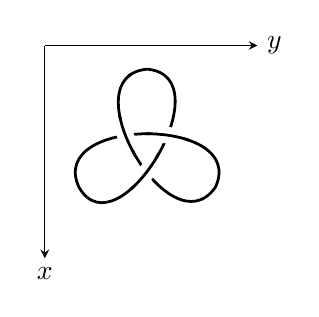
\begin{tikzpicture}
  \draw[-stealth] (0,0) -- (2.7,0) node[right] {$y$};
  % \draw[-stealth] (0,0,0) -- (0,3,0) node[above] {$z$};
  \draw[-stealth] (0,0) -- (0,-2.7) node[below] {$x$};
  \begin{scope}[shift={(1.3,-1.3)}]
    \begin{knot}[
      consider self intersections=true,
      ignore endpoint intersections=false,
      % draft mode=crossings,
      every strand/.append style={line width=1pt},
      flip crossing=3,
      clip width=6,
      clip radius=6pt,
      % background color=red,
    ]
    \strand (0,1)
    .. controls +(185:1) and +(235:1) .. (-30:1)
    % node[below right] {$\Pr(\mathrm{Im}\, K)$}
    .. controls +(65:1) and +(115:1) .. (210:1) 
    .. controls +(300:1) and +(-5:1) .. (0,1);
    \end{knot}
  \end{scope}
\end{tikzpicture}
\end{document}